\documentclass[12pt, a4paper]{article}
% NMD=Not Miktex default

% Margins
\usepackage[top=35mm, bottom=20mm, left=15mm , right=15mm]{geometry}

% Encoding
\usepackage[utf8]{inputenc}
\usepackage[T1]{fontenc}
\usepackage{lmodern}

% Maths
\usepackage{amsmath,amssymb,amsfonts}
%\usepackage{empheq} % NMD

% Extras
%% \usepackage[tight]{shorttoc}
\usepackage{listings} % to dispaly source code
\usepackage{graphicx}
\usepackage{subfigure}
%\usepackage{alltt}
%\usepackage{moreverb}
%\usepackage{multirow}
%\usepackage{makeidx}
%\usepackage{eurosym}

%\usepackage{lmodern}
%\usepackage{setspace} %NMD
%\usepackage{xcolor} %NMD
%\usepackage{lettrine} %NMD
%\usepackage{lipsum} %NMD

% Local
\usepackage[frenchb]{babel}

% PDF Bookmarks (needs .aux and .out files + 2 compilations)
\usepackage[bookmarks=true, colorlinks=true, urlcolor=blue, breaklinks=true]{hyperref}
%% \usepackage{breakurl}

% Graphics
\graphicspath{{pictures/}}

%%%%%%%%%%%%%%%%%%%%%%%%%%%%%%%%%%%%%%%%%%%%%%%%%

% Let's display some code.
\lstset{ %
language=C,                  % choose the language of the code
basicstyle=\ttfamily\small,       % the size of the fonts that are used for the code
%numbers=left,                   % where to put the line-numbers
numberstyle=\footnotesize,      % the size of the fonts that are used for the line-numbers
stepnumber=2,                   % the step between two line-numbers. If it's 1 each line will be numbered
numbersep=5pt,                  % how far the line-numbers are from the code
backgroundcolor=\color{white},  % choose the background color. You must add \usepackage{color}
showspaces=false,               % show spaces adding particular underscores
showstringspaces=false,         % underline spaces within strings
showtabs=false,                 % show tabs within strings adding particular underscores
frame=single,	                % adds a frame around the code
tabsize=8,	                % sets default tabsize to 2 spaces
captionpos=t,                   % sets the caption - b = position to bottom, t = top.
breaklines=true,                % sets automatic line breaking
breakatwhitespace=false,        % sets if automatic breaks should only happen at whitespace
title=\lstname,                 % show the filename of files included with \lstinputlisting; also try caption instead of title
% escapeinside={/?}{?)},         % if you want to add a comment within your code
% columns=flexible,
escapechar=?
}

%%%%%%%%%%%%%%%%%%%%%%%%%%%%%%%%%%%%%%%%%%%%%%%%%

\newcommand{\definition}[2]{\paragraph{#1 \\ \\}\fbox{\begin{minipage}{\textwidth }#2\end{minipage}}}



\newcommand{\fonction}[5]{
\begin{tabular}{rl}
    #1$\colon$ #2 & $\longrightarrow$ #3 \\
             #4 & $\longmapsto$ #5
\end{tabular}
}

%%%%%%%%%%%%%%%%%%%%%%%%%%%%%%%%%%%%%%%%%%%%%%%%%

\begin{document}

\title{Les Textures Procédurales}
\author{Pierre \bsc{Neidhardt}}
\date{4 juin 2010} 
%Version 10.02.28

%%%%%%%%%%%%%%%%%%%%%%%%%%%%%%%%%%%%%%%%%%%%%%%%%
\maketitle

%% \shorttableofcontents{Sommaire}{3}
\tableofcontents
%%%%%%%%%%%%%%%%%%%%%%%%%%%%%%%%%%%%%%%%%%%%%%%%%

%%%%%%%%%%%%%%%%%%%%%%%%%%%%%%%%%%%%%%%%%%%%%%%%%
\pagebreak
%%%%%%%%%%%%%%%%%%%%%%%%%%%%%%%%%%%%%%%%%%%%%%%%%

\subsection{Interpolation}

\subsubsection{Interpolation linéaire}

Fonction d'interpolation linéaire entre $a$ et $b$ :

\[
\boxed{
\fonction {$f$} {$[0;1]$} {$[a;b]$} {$x$} {$a \cdot (1-x) + b \cdot x$}
}
\]

\begin{figure}[!h]
	\centering
	   \caption{Interpolation linéaire en niveau de gris}
	   \bigskip
	   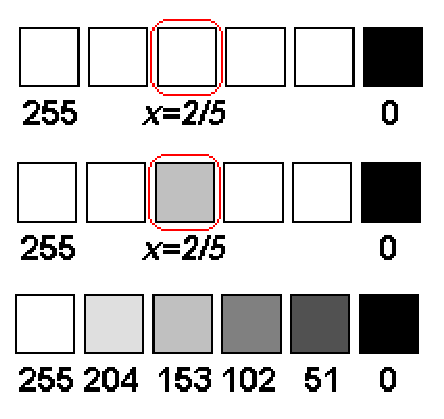
\includegraphics[scale=1]{interpolation}
\end{figure}

%%%%%%%%%%%%%%%%%%%%%%%%%%%%%%%%%%%%%%%%%%%%%%%%%
\pagebreak
%%%%%%%%%%%%%%%%%%%%%%%%%%%%%%%%%%%%%%%%%%%%%%%%%

\subsubsection{Interpolation bilinéaire}

\begin{figure}[h]
	\centering
	   \caption{Procédé d'interpolation bilinéaire}
	   \bigskip
	   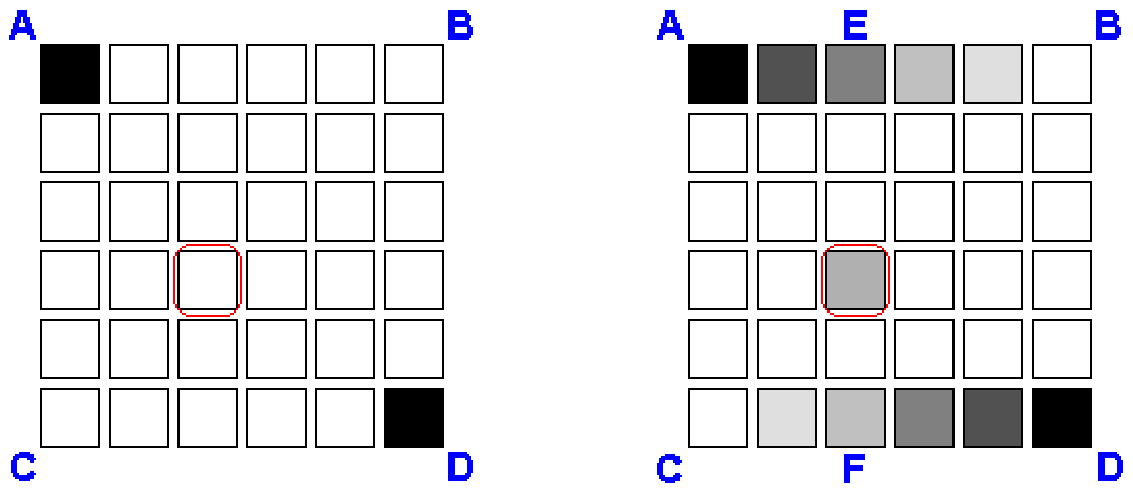
\includegraphics[scale=1]{interpolation_bil}
\end{figure}


\begin{figure}[!h]
  \centering
  \caption{Interpolation bilinéaire}
  \bigskip
  \subfigure[Points d'interpolation en 2D]{\label{fig:contour-a}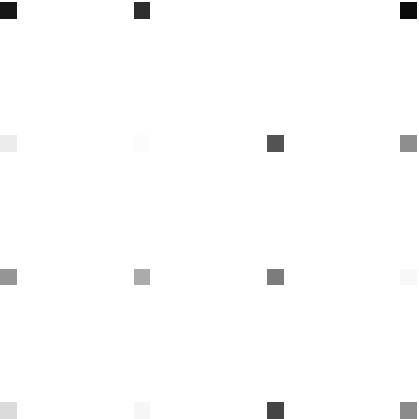
\includegraphics[scale=0.75]{interpol_bil_step1}}
  \subfigure[Application de l'interpolation bilinéaire]{\label{fig:contour-b}
\includegraphics[scale=1]{interpol_bil_step2}}
\end{figure}

%%%%%%%%%%%%%%%%%%%%%%%%%%%%%%%%%%%%%%%%%%%%%%%%%
\clearpage
%%%%%%%%%%%%%%%%%%%%%%%%%%%%%%%%%%%%%%%%%%%%%%%%%
\subsubsection{Fonctions d'interpolation non linéaire}

Interpolation cosinusoïdale entre $a$ et $b$ :

\[\boxed{
\fonction{$f$}{$[0;1]$}{$[a;b]$}{$x$}{$a \cdot \frac {1+\cos(x\cdot\pi)} {2} + b \cdot \frac {1-\cos(x\cdot\pi)} {2}$}
}\]

\begin{figure}[!h]
	\centering
	   \caption{Interpolation cosinusoïdale}
	   \bigskip
	   
\includegraphics[scale=1]{interpol_cos}
\end{figure}


%%%%%%%%%%%%%%%%%%%%%%%%%%%%%%%%%%%%%%%%%%%%%%%%%
\clearpage
%%%%%%%%%%%%%%%%%%%%%%%%%%%%%%%%%%%%%%%%%%%%%%%%%

\bigskip
\begin{lstlisting}[caption=Code C - Interpolation non linéaire]
int interpol(int y1, int y2, int n, int espace){

    if (n==0) return y1;
    if (n==1) return y2;

    double x = (double) espace/n;

    double facteur1 = 3*pow(1-x, 2) - 2*pow(1-x,3);
    double facteur2 = 3*pow(x, 2) - 2*pow(x, 3);

    return y1*facteur1 + y2*facteur2;
}

int interpol_val(int i, int j, int frequence, calque *c){

    // Position des points d'interpolation.
    int x1, x2, y1, y2, position;
    float pas;
    pas = (float)c->taille/frequence;

    position = (float)i/pas;
    x1 = position*pas;
    x2 = (position+1)*pas;
    if(x2 >= c->taille) x2 = c->taille-1;

    position = (float)j/pas;
    y1 = position*pas;
    y2 = (position+1)*pas;
    if(y2 >= c->taille) y2 = c->taille-1;

    int valeur11, valeur12, valeur21, valeur22;
    valeur11 = c->v[x1][y1];
    valeur12 = c->v[x1][y2];
    valeur21 = c->v[x2][y1];
    valeur22 = c->v[x2][y2];

    int valeurA = interpol(valeur11, valeur12, y2-y1, j-y1);
    int valeurB = interpol(valeur21, valeur22, y2-y1, j-y1);
    int valeur_finale = interpol(valeurA, valeurB, x2-x1 , i-x1);

    return valeur_finale;
}

\end{lstlisting}

\bigskip
Interpolation polynomiale : PB avec Runge.

\bigskip
Interpolation cubique : meilleure solution (fonctions splines)

%%%%%%%%%%%%%%%%%%%%%%%%%%%%%%%%%%%%%%%%%%%%%%%%%
\clearpage
%%%%%%%%%%%%%%%%%%%%%%%%%%%%%%%%%%%%%%%%%%%%%%%%%

\subsection{Fusion des différentes interpolations}

\subsubsection{Définitions}

\definition{Fréquence}{Nombre de pixels utilisés comme points d'interpolation (sur une seule dimension). Ces pixels sont séparés par un interval constant appelé \textbf{pas}, dépendant de la fréquence et de la taille de l'image.}

\begin{figure}[h]
	\centering
	   \caption{Fréquence}
	   \bigskip
	   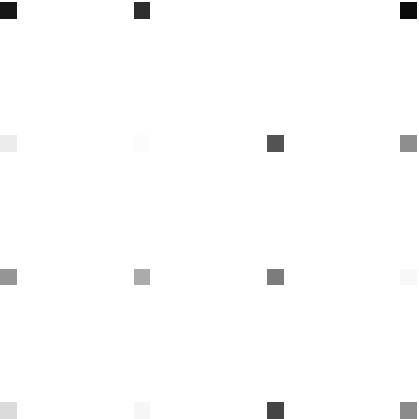
\includegraphics[scale=0.8]{interpol_bil_step1}
\end{figure}

\definition{Octave}{Calque dessiné en parallèle à l'image de base avec un certaine fréquence. Tout calque a une fréquence supérieure à celle du calque précédent (typiquement le carré de la fréquence de celle-ci). Le calque est fusionné avec l'image de base pour donner le résultat final.}

\definition{Persistance}{Facteur de pondération associé à un calque lui conférant plus ou moins d'importance sur le résultat final.}

\bigskip
Remarque : comme les valeurs du calque doivent rester dans $\{0;255\}$, il faut prendre garde que la somme totale ne dépasse pas 255, sans quoi  cela donne lieu à des incohérences.
Une persistance maximale de 0.5 assure l'absence d'incohérence :
\[
	\sum_{k=1}^{\infty} p^k= \frac {p} {1-p} \leqslant 1 \Rightarrow p \leqslant 0.5
\]

\bigskip
Paramètres de la texture :
\begin{itemize}
	\item $\mathbf{graine} \in \mathbb{N}$
	\item $\mathbf{frequence} \in \{ 2^i; i \in \mathbb{N}\}$
	\item $\mathbf{nombre\_octaves} \in \mathbb{N}$
	\item $\mathbf{persistance} \in [0,1]$
\end{itemize}


%%%%%%%%%%%%%%%%%%%%%%%%%%%%%%%%%%%%%%%%%%%%%%%%%

\end{document}
